\documentclass[11pt]{amsart}
\usepackage{geometry}                % See geometry.pdf to learn the layout options. There are lots.
\geometry{letterpaper}                   % ... or a4paper or a5paper or ... 
%\geometry{landscape}                % Activate for for rotated page geometry
%\usepackage[parfill]{parskip}    % Activate to begin paragraphs with an empty line rather than an indent
\usepackage{graphicx}
\usepackage{amssymb,tikz}
\usepackage{epstopdf}
%\usepackage{multicolumn}
\usepackage{tabularx}
\usepackage{subcaption}
\DeclareGraphicsRule{.tif}{png}{.png}{`convert #1 `dirname #1`/`basename #1 .tif`.png}

\title{Methods}
\author{Nick Kappler}


\begin{document}
\maketitle
\section{Including Parasites (or, changing a few body size ratios)}


\subsection{Niche Models\label{sec:structure}}

We first generated 100 food webs with 40 species and connectance $C=0.15\pm .0075$ using the Niche Model.  The Niche model is an algorithm that generates realistic food webs with minimal inputs.\footnote{'We looked at alternatives but they did not pass muster.' Keep this in your backpocket.}  Figure \ref{fig:nicheModel} shows the procedure.  A species, $j$ is placed on the niche axis, $[0,1]$, bu choosing a niche value uniformly randomly from $[0,1]$.  This species is then given a diet center, and diet width.  The diet width has two components.  The first, $y_j$, is drawn from a beta distribution with $\alpha = 1$, and $\beta$ chosen so that the expected width of a diet is the desired connetance, $C$.  The beta distribution is chosen so that the distribution of diet widths is approximately exponential, which means the distribution of generalities will be approximately exponential.  This value is then multiplied by $n_j$ so that species with higher niche values will tend to be more generalist than species with lower niche values (the range of $j$ is $r_j = n_jy_j$.  A diet center, $c_j$, is chosen uniformly randomly such that $c_j \leq n_j$ and the diet falls entirely within the niche axis.  Species $j$ consumes a species $i$, if $n_i$ falls within the feeding range of $j$.  


\begin{figure}{h}
%This is a schematic of the Niche Model.
\begin{tikzpicture}
\draw (0,0)--(10,0)
node[anchor = west] {$n$};
\draw (0,.2)--(0,-.2)
node[anchor = north] {$0$};
\draw (10,.2)--(10,-.2)
node[anchor = north] {$1$};
%Predator
\fill (7,0) circle (.07) 
node[anchor = north]  {$n_j$};
%Predator Diet
\draw (7,0)--(7,.75)--(2,.75)--(2,.5);
\draw (.3,0) -- (.3,.5) -- (3.7,.5) -- (3.7,0);
\draw[dashed] (2,.5) -- (2,0) 
node[anchor = south east] {$c_j$};
\draw[<->] (.3,-.5) -- (3.7,-.5)
node[fill=white,pos = 0.5] {$r_j$}; 
\draw[dashed] (.3,0)--(.3,-.55);
\draw[dashed] (3.7,0)--(3.7,-.55);
%Prey
\fill (3,0) circle (.07) 
node[anchor = north west]  {$n_i$};
\draw(4.2,-2) circle (.3)
node {$i$};
\draw[->] (4.5,-2) -- (5.5,-2);
\draw(5.8,-2) circle (.3)
node {$j$};
\end{tikzpicture}
\caption{This figure demonstrates how feeding relationships are determined in the Niche Model.\label{fig:nicheModel}}
\end{figure}

\subsection{Allometric Trophic Network Model}

We simulated population dynamics on the food web structures described in section \ref{sec:Structure} using the Allometric Trophic Network (ATN) model.  The ATN model is an easily parameterized and extensible model that has been shown to be capable of accurately reproducing real dynamics \cite{Boit2012}.  At the heart of the ATN model is the assumption that a species' metabolic rate is a species most fundamental constant.  It affects mortality and biomass accumulation.  The dependence on this fundamental biological rate means that the only species-specific parameter needed is body size.  We use the following formula to generate body sizes for any free-living species within a network structure:
\begin{equation}
M_i= Z_f^{TL_i-1}\label{eq:MFree}
\end{equation}

Where $TL_i$ is the prey-averaged trophic level of species $i$ and $Z_f$ is a constant that represents the average of the log of the body size ratio of consumer $i$ to its prey.  $Z_f$ will therefore determine the average body size ratio of the entire food web.  Using this body size, we define the mass-specific metabolic rate as
\begin{equation}
x_i = a_x_i M_i^{-0.25}\label{eq:x}
\end{equation}
The $-0.25$ power has both empirical and theoretical support (REFS).  The constant $a_x_i$ is the metabolic scaling constant that varies across metabolic classes of species.  In all simulations we take $a_x_i=0.314$, which is the value for a broad collection of invertebrate species.  With these fundamental constants in hand we can write the following dimensionless equations that govern the biomasses of all species in a food web (see \cite{Yodzis1992} and \cite{Willams2007} for full derivations): 

\begin{align}
\frac{dB_{b}}{dt} &= r_bB_b\left(1-\frac{\sum_{k\in\text{basal}}B_k}{K}\right) - \sum_kB_kx_k\frac{y_{bk}F_{bk}}{e_{bk}}\label{eq:basal0} \\ 
\frac{dB_{c}}{dt} &= -x_cB_c + x_cB_c\sum_ky_{kc}F_{kc} - \sum_k x_kB_k\frac{y_{ck}F_{ck}}{e_{ck}} \label{eq:con0}
\end{align}

Here $B_b$ and $B_c$ denote biomass density of basal and consumer species; thus \eqref{eq:basal0} and \eqref{eq:con0} represent rates of change of basal and consumer populations, respectively (regardless of whether the consumer is a free liver or parasite).  $r_b$ is the growth rate of basal species $b$ and $K$ is the shared system carrying capacity of all basal species.  $x_i$ is the mass specific metabolic rate of consumer $i$. $y_{ij}$ is the maximum assimulation rate of $i$ by $j$ relative to $j$'s metabolic rate and $e_{ij}$ is the assimilation efficiency of $j$ when consuming $i$. $F_{ij}$ is the functional response of $j$ preying on $i$ and has the following form:
\begin{equation}
\frac{\omega_{ij}B_j^{1+q}}{B_0^{1+h} + \sum_k\omega_{kj}B_k^{1+h}}\label{eq:FR0}
\label{fr0}
\end{equation}
Here $h$ quantifies deviation from a multi-species type II functional response, $\omega_{ij}$ is the relative preference for prey item $j$ by $i$, and $B_0$ is the half-saturation density.  When $h=0$ and $j$ has only one prey, this is the density of prey that yields an attack rate on $i$ by $j$ equal to half the maximum attack rate.  In the case of multiple prey or $h\neq0$, it is harder to interpret but generally affects how quickly the functional response approaches its saturating value.  

\subsection{Introducing Parasites}

We controlled the number of parasites in our food webs by switching the roles of randomly selected consumers from free-living species to parasitic species.  In this study, the most basic difference between a free-living consumer and a parasitic consumer is the body size ratio of the parasite to its host species.  On average, a parasitic species will be much smaller than its host, whereas a free-living consumer will generally be much larger than its prey.  When a consumer is chosen to be a parasite, we determine its body size by the following formula:
\begin{equation}
M_i = 10^{p + k(TL_i -2)} \label{eq:Mpara}
\end{equation}

With this choice, parasites will on average be $10^{p}$ times the size of their free-living hosts, $10^k$ times larger than their parasitic prey (same as free-livers on free livers; note that $k = \log Z_f$) and $10^{2k-p}$ times smaller than their free-living predators.  The last ratio ($10^{2k-p}$) is not ideal since it significanty increases the average body size ratio of free-living consumers.  From the parasitic body sizes we derive mass-specific metabolic rate using equation \ref{eq:x}.

We chose a sequence of parasites to add to each food web (that is, chose consumers to be parasites) uniformly randomly and used the same sequence for each simulation in each web.  The sequence is used so that the parasites at a given level of parasitism are a subset of the parasites at a higher level of parasitism.  We judged this to be the best way to test the effect of increasing the level of parasitism since it controlled the random effect of particularly disruptive parasites.  This also alowed for more direct comparisons between models.  Ideally we would have tested many sequences of parasites for each web, but we were limited by computing resources at the time of this study.  




%This is a schematic for concomittant predation.
\begin{figure}
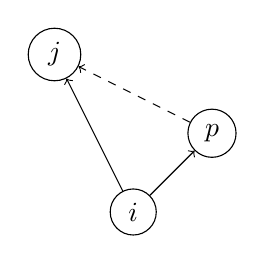
\begin{tikzpicture}
\node[draw,circle] at (0,0) (j) {$j$};
\node[draw,circle] at (1,-2) (h) {$i$};
\node[draw,circle] at (2,-1) (p) {$p$};
\draw[->] (h)--(j);
\draw[->] (h)--(p);
\draw[->,dashed] (p)--(j);
\end{tikzpicture}
\caption{This diagram illustrates concomittant predation.  The biomass of $p$ that is inside host $h$ is consumed when $h$ is eaten by its consumer, $j$. \label{fig:concDiagram}}
\end{figure}

(for a total of $4\times2\times2\times 11\times 100 = 17600$ simulations).  


Each type of species (free-liver and parasite) will be tested with two different body size ratios: free livers will be 10 times larger than their prey, on average, for one set of simulations, and 100 in another set.  Likewise, parasites will be on average 1,000 or 10,000 times smaller than their host.  This can lead to some problems - see the issues section.  These two factors lead to 4 sets of simulations.

I will further test two additional pieces to the model.  The first is including a constant for each species that represents the fraction of the population in a free living stage.  I denote this constant $\phi_{i}$ (equal to 1 for free-living specie).  I use this constant to split the parasites interaction into trophic and non-trophic (i.e. parasite-host) interactions.  Parasites are only vulnerable to predation (or parasitism) during their free-living stage.  When they are inside a host ($1-\phi_{i}$ of the population), they are only vulnerable to concomitant predation.\footnote{But note that parasites should be able to eat each other inside hosts as well.  Also, some parasites can be eaten by symbionts of their host - i.e. pilot or remora fish and sharks.}  The second addition to the model is concomitant predation.  When a parasite is in a host, it is killed when that host is eaten.  At this point, the benefit to the consumer will be neglected.  See below for explicit formulae.  These two models will be added one at a time to a basic ATN model which gives 4 different models (no addition, just fraction free-living, just concomitant, fraction free-living and concomitant).


\subsection{Models}
I will be using 4 models.  The basic ATN model is as follows (see the parameters section for parameter values):

\begin{figure}
\begin{subfigure}{.45\textwidth}
\caption{Null Model\label{subfig:modelsA}}
\includegraphics[width=\textwidth]{../figures/Null.png}
\end{subfigure}
\begin{subfigure}{.45\textwidth}
\caption{refuge\label{subfig:modelsb}}
\includegraphics[width=\textwidth]{../figures/Null+Ref.png}
\end{subfigure}

\begin{subfigure}{.45\textwidth}
\caption{concomittant\label{subfig:modelsc}}
\includegraphics[width=\textwidth]{../figures/Null+Con.png}
\end{subfigure}
\begin{subfigure}{.45\textwidth}
\caption{refuge with concomittant\label{subfig:modelsd}}
\includegraphics[width=\textwidth]{../figures/Con+Ref.png}
\end{subfigure}
\caption{This cartoon illustrates the differences between the four different versions of ATN dynamics that were tested.  \label{fig:cartoons}}
\end{figure}

In the first model (figure \ref{subfig:modelsA}) parasites are vulnerable to their predators while both inside and outside their hosts and they are not susecptible to concomittant predation.  In this model, the only things that change when a species becomes a parasite are it's body size and metabolic rate.  In the second model, (figure \ref{subfig:modelsB})  we introduce a parameter, $\phi$, to the null model that controls the fraction of parasitic biomass outside of a host at any given time.  A parasite is protected from predation while inside of its host.  However, the parasite is also not susceptible to concomittant predation.  This represents the situation in which parasites are most protected.  The third model (figure \ref{subfig:modeslsC}) modifies the null model by making parasites within their hosts susceptible to concomittant predation.  Note that in this model we don't distinguish where a parasite is; so the entire popluation is suscpetible to concomittant predation and normal predation.  This model represents the most vulnerable state for parasites.  In the final model (figure \ref{subfig:modelsD}) we use the parameter $\phi$ to determine what fraction of parasitic biomass is susceptible to concomittant predation.  The fraction of parasitic biomass that is inside a host is protected from standard predation.  This was designed to be the most 'realistic' situation.


\begin{equation}
\phi_i = 
\left\{
\begin{array}{c c c}
\phi & \text{if} & i:\text{ parasite}\\
1 & \text{if} & i:\text{ free-liver}\\
\end{array}
\right.\label{phidef}
\end{equation}
note that this means in particular that $\phi_i$ is the same for all parasites and 1 for all free-livers.  using $\phi_i$  i make the following changes to \eqref{eq:basal0} and \eqref{eq:con0}:

\begin{align}
\frac{db_{b}}{dt} &= r_bb_b\left(1-\frac{\sum_{k\in\text{basal}}b_k}{k}\right) - \sum_k\phi_kb_kx_k\frac{y_{bk}f_{bk}^\text{(troph)}}{e_{bk}} - \sum_k(1-\phi_k)b_kx_k\frac{y_{bk}f^\text{(para)}_{bk}}{e_{bk}}\label{basaleq1} \\ 
\frac{db_{c}}{dt} &= -x_cb_c + \phi_cx_cb_c\sum_ky_{kc}f^\text{(troph)}_{kc} + (1-\phi_c)x_cb_c\sum_ky_{kc}f^\text{(para)}_{kc} \label{coneq1}\\ 
&- \sum_k \phi_kx_kb_k\frac{y_{ck}f^\text{(troph)}_{ck}}{e_{ck}} - \sum_k (1-\phi_k)x_kb_k\frac{y_{ck}f^\text{(para)}_{ck}}{e_{ck}}\nonumber
\end{align}

though a lot more ink (or pixels) is required to write down this model, the basic idea is simple: i split the links to parasites by whether or not the parasite acts as a classic consumer (larger than prey) or a parasitic consumer (smaller than prey), then treat them appropriately.  to do this, i needed to introduce two separate  preference matrices, $\omega_{ij}$, and therefore two separate functional response, namely:

\begin{equation}
f_{ij}^\text{(troph)} = \frac{\omega_{ij}^{(troph)}(\phi_ib_i)^{1+h}}{b_0^{1+h} + \sum_k\omega^\text{(troph)}_{kj}(\phi_kb_k)^{1+h}} \label{fr1troph}
\end{equation}
and
\begin{equation}
f_{ij}^\text{(para)} = \frac{\omega_{ij}^{(para)}(\phi_ib_i)^{1+h}}{b_0^{1+h} + \sum_k\omega^\text{(para)}_{kj}(\phi_kb_k)^{1+h}} \label{fr1para}
\end{equation}

two changes have been made to the original functional response.  first, all prey biomasses (in both functional response) have been multiplied by the fraction of free living time.  this is because only the portion $\phi_i$ of the biomass of species $i$ is available for consumption (either by free-livers or parasites) at any given time.  second, the preference for a particular species is now determined by $\omega_{ij}^\text{(troph)}$ in $f_{ij}^\text{(troph)}$ and $\omega_{ij}^\text{(para)}$ in $f_{ij}^\text{(para)}$.  these new preferences take into account the fact that a parasite does not have to divide its foraging time as a free liver among its hosts.  by the same token, it doesn't have to divide it's 'foraging' time among it's free-living (i.e. trophic) prey items when within a host.

the second addition is concomitant predation on parasites.  this comes in as an added term subtracted at the end of equations \eqref{eq:con0} or \eqref{coneq1}.  the term can be compactly expressed as 
\begin{equation}
i_p = \sum_ha_{ph}c_h \label{ip1}
\end{equation}
where $a_{ph}$ is the biomass of parasite $p$ per unit of biomass of host $h$, and $c_h$ is the total trophic consumption (total rate of change) of host $h$.  breaking it down, we have
\begin{equation}
a_{ph} = \frac{(1-\phi_p)b_p}{b_h}\frac{y_{hp}f^\text{(para)}_{hp}}{\sum_{k}y_{kp}f^\text{(para)}_{kp}} \label{aph1}
\end{equation}
when we separate the trophic and parasitic links of parasites, and
\begin{equation}
a_{ph} = \frac{b_p}{b_h}\frac{y_{hp}f_{hp}}{\sum_{k}y_{kp}f_{kp}} \label{aph2}
\end{equation}
when we treat all links to parasites as parasitic.  in \eqref{aph1} and \eqref{aph2}, i have defined the fraction of the biomass of parasite $p$ in host $h$ to be the ratio of parasite $p$'s (parasitic) attack rate on $h$ divided by it's total (parasitic) attack rate on all of $h$'s hosts.  finally,
\begin{equation}
c_h = \sum_kx_kb_k\frac{f^\text{(troph)}_{kh}y_{kh}}{e_{kh}} \label{cpheq}
\end{equation}
so, putting it all together we have
\begin{equation}
i_p = \sum_h \left(\frac{b_p}{b_h}\frac{y_{hp}f_{hp}}{\sum_{k}y_{kp}f_{kp}}\left[\sum_kx_kb_k\frac{f^\text{(troph)}_{kh}y_{kh}}{e_{kh}}\right] \right) \label{ip2}
\end{equation}

\subsection{parameter values}
all simulations are run on niche model webs with $s = 40$ and $c = 0.15$.  in the atn model, most parameters are found via allometric scaling relationships.  body mass is then one of the most fundamental parameters.  since i want to test the effect of different body size ratios in this model, i define body mass for free-livers as follows:

\begin{equation}
m_i = z_i^{t_i-1} \label{mf}
\end{equation}


where $z_i=z$ is the desired body mass ratio for free-livers, and $t_{i}$ is the trophic level of species $i$.  in my simulations i use the short-weighted trophic level.  thus, if i want predators to be, on average, 10 times larger than their prey, i would set $z = 10$.  if i desired 100 times larger, i would use $z=100$.  unfortunately it does not work so simply for parasites.  to describe how parasite body masses are determined i need a few more parameters. define $k$ as the common logarithm of the consumer-resource body size (c-r bsr) ratio for free livers, and $p$ as the common logarithm of the desired  c-r bsr for parasites preying on hosts.  then if we set the body size for parasites as 


\begin{equation}
x_i = a_xm_i^{-1/4}\label{xeq}
\end{equation}

for all my simulations i take $a_x = 0.314$, the constant for invertebrates.  see the table below for the remaining parameter values.

in the functional response, i use the strong generalist model, so $\omega_{ij} = 1 \forall i,j$.  i also use a 'type ii.2' functional response, so $h = 0.2$.  finally, i use $B_0 = 0.5$ (all from brose, williams, and martinez 2006).

many of the other constants in the models are determined from allometry, though the actual values are simply taken to be consistent with other papers since they are defined such that they scale with $x_i$.  All parameters are summarized in the table below.

\begin{table}
\begin{tabularx}{\textwidth}{|l|X|l|}
\hline
\multicolumn{3}{|X|}{Allometric Parameters}\\
\hline
Parameter&Description&Value\\
\hline
$a_x^{(inv)}$&Scaling constant for metabolic rate of invertebrate consumers & $0.314$\\
$z$&Consumer-resource body size ratio&variable, $n=4$\\
\hline
\hline
\multicolumn{3}{|X|}{Functional Response Parameters}\\
\hline
Parameter&Description&Value\\
\hline
$b_0$&Half-saturation density&$0.5$\\
$h$&Hill coefficient modifier& $0.2$\\
$\omega_{ij}$&Preference of $i$ for $j$&$1$ or $0$\\
\hline
\hline
\multicolumn{3}{|X|}{ATN Parameters}\\
\hline
Parameter&Description&Value\\
\hline
$r_i$&Intrinsic growth of producer $i$&$\mathcal{N}(1,0.1)$\\
$K$&Community carrying capacity of producers &5\\
$x_i$&Metabolic rate of consumer $i$&$a_x m_i^{-0.25}$\\
$y_i$&Maximum rate of assimilation relative to metabolic rate for invertebrate consumers & 8\\
$e_{ij}^{(carn.)}$&Assimilation efficiency of $j$ by $i$ for a consumer $j$ (carnivory) & 0.85\\
$e_{ij}^{(herb.)}$&Assimilation efficiency of $j$ by $i$ for a producer $j$ (herbivory) & 0.45\\
\hline
\hline
\multicolumn{3}{|X|}{Food Web Parameters}\\
\hline
Parameter&Description&Value\\
\hline
$s$&Species richness&40\\
$c$&Connectance & 0.15\\
\hline
\hline
\multicolumn{3}{|X|}{Independent Variables}\\
\hline
Parameter & Values or Description & Replicates\\
$z_\text{free}$&$z=10,100$&2\\
$z_\text{para}$&$z=.001,.0001$&2\\
$i_p$&concomittant loss (y/n)&2\\
$\phi$&Differentiate parasitic biomasses inside and outside hosts (y/n)&2\\
$f_{par}$&Fraction of consumers as parasites (evenly spaced between 0 and .5)&11\\
\hline
\end{tabularx}
\caption{Values of all constants used in the models.  \label{tab:param}}
\end{table}
\newpage

\end{document}  
